\documentclass[a4paper]{article}

\usepackage{amsmath}
\usepackage{amssymb}
\usepackage{parskip}
\usepackage{fullpage}
\usepackage{hyperref}
\usepackage{bettelini}
\usepackage{stellar}
\usepackage{graphicx}
\usepackage{tikz}
\usepackage{fancybox}
\usepackage{makecell}
\usepackage[backend=bibtex]{biblatex}

\hypersetup{
    colorlinks=true,
    linkcolor=black,
    urlcolor=blue,
    pdftitle={Chemistry},
    pdfpagemode=FullScreen,
}

\addbibresource{./references.bib}

\title{Chimica}
\author{Paolo Bettelini}
\date{}

\begin{document}

\maketitle
\tableofcontents

% 978.88.08.72527.1
% CHIMICA.BLU J.Brady

\pagebreak

\section{Chimica}

Sistema \(\subseteq\) Ambiente \(\subseteq\) Universo.

Un sistema può essere:
\begin{itemize}
    \item \textbf{Aperto:} se scambia materia/energia con l'ambiente.
    \item \textbf{Chiuso:} se scambia solo energia con l'ambiente.
    \item \textbf{Isolato:} se non scambia nè energia nè material con l'ambiente.
\end{itemize}

Studiare un sistema significa descrivere le sue proprietà
\begin{itemize}
    \item \textbf{Qualitative:} possono essere definite senza avvalersi
    di misure.
    \item \textbf{Quantitative:} richiedono delle misure.
\end{itemize}
Le priorità misurabili sono delle \textit{grandezze}.

% TODO intensive / estensive

\subsection{Notazione scientifica}

La notazione scientifica viene espressa come
\[
    a \cdot 10^k,\quad a\in [1, 10)
\]

\subsection{Sistema Internazionale}

\subsubsection{Grandezze fondamentali}

\begin{figure}[h]
    \centering
    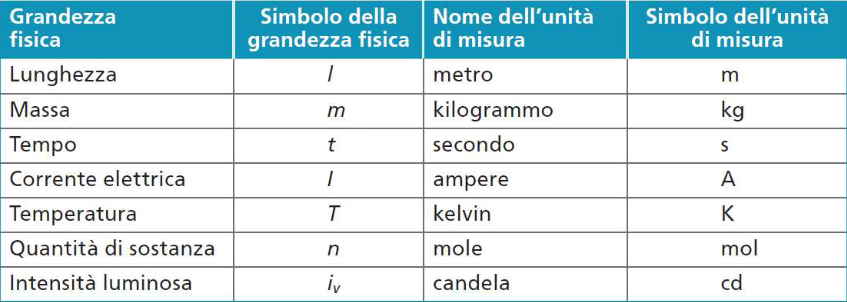
\includegraphics[width=0.75\textwidth]{./si.png}
\end{figure}

\subsubsection{Grandezze derivate}

\begin{figure}[h]
    \centering
    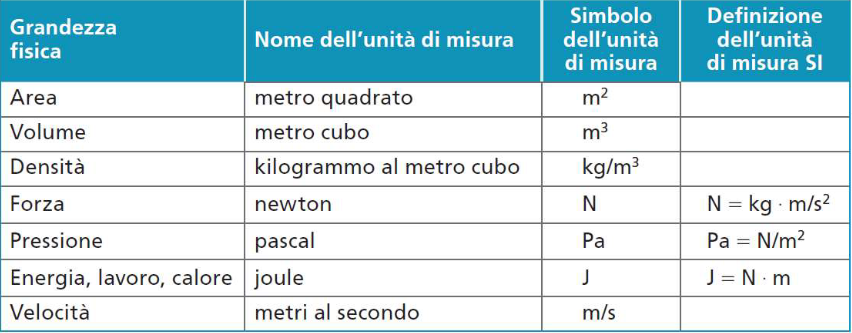
\includegraphics[width=0.75\textwidth]{./grandezzederivate.png}
\end{figure}

\pagebreak

\subsubsection{Misure}

\begin{figure}[h]
    \centering
    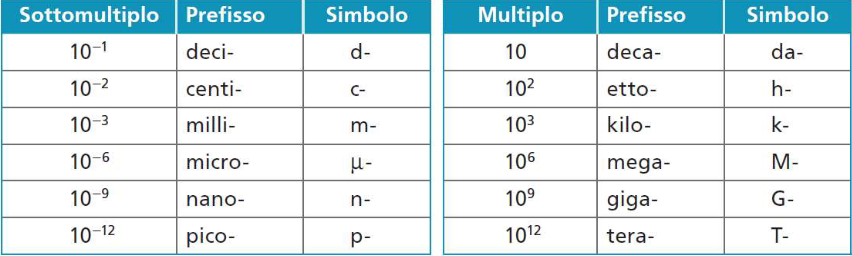
\includegraphics[width=0.75\textwidth]{./misure.png}
\end{figure}

\pagebreak

\section{Trasformazioni}

Le trasformazioni possono essere classificate come \textit{chimiche} o \textit{fisiche}.

\sdefinition{Trasformazione chimica}{
    Una \textit{trasformazione chimica}
    modifica la sostanza.
}

Nelle trasformazioni chimiche, gli atomi sono gli stessi ma gli elementi sono diversi.
Le particelle quindi mutano.

\sdefinition{Trasformazione fisica}{
    Una \textit{trasformazione fisica}
    non modifica la materia ma il suo stato.
}

Nelle trasformazioni fisiche, la materia mantiene le sue proprietà e rimane invariata.

\sexample{Trasformazioni chimiche}{
    \begin{itemize}
        \item Combustione di una candela (anche fisica).
        \item Cottura di un uovo (le proteine cambiano).
        \item Formazione della ruggina.
    \end{itemize}
}

\sexample{Trasformazioni fisica}{
    \begin{itemize}
        \item Combustione di una candela (anche chimica).
        \item Sbucciare una mela.
        \item Scaldare il tisolfato di sofio.
        \item Dissoluzione dello zucchero nell'acqua.
    \end{itemize}
}

\pagebreak

\section{Classificazione}

\subsection{Definizione}

\sdefinition{Sostanza pura elementare}{
    Una \textit{sostanza pura elementare} è composta da un solo tipo di elemento.
}

\sdefinition{Sostanza pura composta}{
    Una \textit{sostanza pura composta} è composta da un solo tipo di composto.
}

\sdefinition{Soluzione}{
    Una \textit{soluzione} è una sostanza composta da diversi tipi di composti
    in maniera omogenea.
}

\sexample{Sostanza pura composta}{
    Acqua (\(H_2O\))
}

\sexample{Sostanza pura elementare}{
    Azoto (\(N\))
}

\sexample{Soluzione}{
    \(50\% N + 50\% H_2\)
}

\begin{center}
    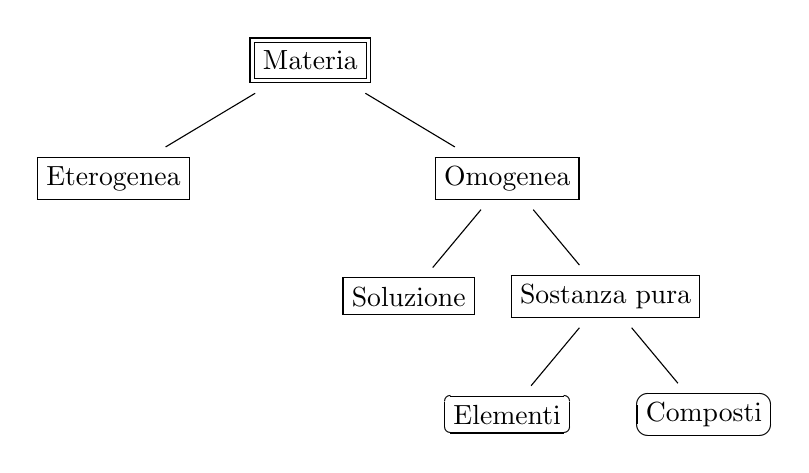
\begin{tikzpicture}[
        level 1/.style = {sibling distance = 5cm},
        level 2/.style = {sibling distance = 2.5cm}
    ]
    \node {\doublebox{Materia}}
        child {
            node {\fbox{Eterogenea}}
        }
        child {
            node {\fbox{Omogenea}}
            child {
                node {\fbox{Soluzione}}
            }
            child {
                node {\fbox{Sostanza pura}}
                child {
                    node {\ovalbox{Elementi}}
                }
                child {
                    node {\ovalbox{Composti}}
                }
            }
        };
    \end{tikzpicture}
\end{center}

\begin{itemize}
    \item La materia può essere classificata come materia \textit{eterogenea}
    e materia \textit{omogenea}.
    
    \item La materia omogenea può essere classificata come \textit{miscuglio omogeneo} (soluzione)
    oppure come \textit{sostanza pura}.
    
    \item Le sostanze pure possono essere classificati come \textit{elementi} oppure \textit{composti}.
\end{itemize}

\pagebreak

\subsection{Soluzioni (miscugli omogenei)}

Ogni soluzione è caratterizzata
da un \textit{soluto} ed un \textit{solvente}.

\sdefinition{Solubilità}{
    La \textit{solubilità} è la quantità massima che una sostanza
    può essere sciolta da una determinata quantità di solvente.
}
La solubilità dipende dalle proprietà chimica e altri fattori come la temperatura.
La solubilità dei gas diminuisce con l'aumento della temperatura.

Una soluzione è detta \textit{satura} o \textit{insatura}
se ha raggiunto il suo quantitativo massimo o meno.

Quando un soluto viene sciolto in un solvente, il volume della soluzione aumenta,
ma meno della somma dei due volumi. Questo è dato dal fatto che il soluto prende spazio fra le molecole del solvente.

\subsection{Tecniche di separazione}

\sdefinition{Decantazione}{
    La \textit{decantazione} si usa di solito per separare due liquidi di densità diversa
    sfruttando la gravità.
}

\sexample{Decantazione}{
    la separazione dell'olio e l'acqua.
}

\sdefinition{Distillazione}{
    La \textit{distillazione} sfrutta i diversi punti di ebollizione di due liquidi per separarli.
    La miscela viene riscaldata fino a quando solo uno delle due componenti diventa vapore, per poi
    spostarla e riaffreddarla.
}

\sdefinition{Cromatografia}{
    La \textit{cromatografia} sfrutta la tendenza delle sostanze a sciogliersi o interagire
    con diverse specie chimiche.
}

\sdefinition{Estrazione}{
    L'\textit{estrazione} si basa sulla maggiore o minore solubilità di un componente di un miscuglio in una certa miscela.
}

\sdefinition{Filtrazione}{
    TODO
}

\sdefinition{Centrifugazione}{
    TODO
}

\pagebreak

%\section{Reazioni chimica}
%Se una reazione chimica fra due elementi ha un rapporto di massa m, il rapporto delle massa atomiche è pari al rapporto, ma contando per il numero di atomi che reagiscono fra di loro.
% Se 1 atomo reasgisce con 1 atomo, il rapporto delle massa del reagente sarà il rapproto delle masse atomiche. 
% Legge delle proporzioni definite e costanti

%\pagebreak

\section{Polarità}

\sdefinition{Polarità}{
    Una molecola è polare (non pura) se vi è una carica parziale.
}
Il legale ionico è quello più polare perché strappa un elettrone. \\
La differenza di elettronegatività deve essere da 0 a 0.45 per essere puro
(il valore 0.45 è scelto per considerare il legame CH come apolare).

Quando una molecola è fatta solo da 2 atomi, 
se il legame è polare, la molecola è polare.
Quando ci sono più legami, è necessario almeno un legame polare
ma la molecola non deve essere simmetrica, altrimenti le cariche parziali si annullano.

Le sostanze apolari si sciolgono in solventi apolari, e quelli polari in quelli polari.
Di conseguenza, oer essere solubile in acqua una moecola deve essere polare.


\section{Lgami secondari (forze intermolecolari)}

\sdefinition{Forza forte}{
    Legame covalente, metallico o ionico.
}
\sdefinition{Forza debole}{
    Forze di Van der Walls, forze di Londom, ponte a idrogeno.
}

I legami secondari (deboli, intermolecolari) sono responsabili delle interazioni fra molecole uguali o diverse tra loro,
o anche fra parti diverse della stessa molecola.

Se il legame non è un ponte idrogeno ma è lo stesso principio, di dice dipolo-dipolo.
Infatti, il legame ponte idrogeno è dipolo-dipolo ma ha un nome speicfico.
Le forze di Van der Walls sono i legami dipolo-dipolo.
Quando le interazioni non sono polari si parla di forze di London.

\pagebreak

\section{Isotopi dell'idrogeno}

\subsection{Deuterio}

Il primo isotopo dell'idrogeno è il \textit{deuterio}, indicato con \(D\) o \(^2H\).
A differenza dell'idrogeno comune, il deuterio possiede un neutrone nel nucleo oltre al protone.
A causa di questa caratteristica, il deuterio ha una massa atomica leggermente superiore rispetto all'idrogeno normale.
Il deuterio è utilizzato in varie applicazioni, come nei reattori nucleari per la produzione di energia e come tracciatore in studi scientifici e biologici. 

\subsection{Trizio}

Il secondo isotopo dell'idrogeno è è il trizio, indicato con \(T\) o \(^3H\).
A differenza dell'idrogeno comune, il deuterio possiede due neutroni nel nucleo oltre al protone.
A causa di questa composizione nucleare, il trizio ha una massa atomica maggiore rispetto agli altri isotopi dell'idrogeno.
Il trizio è radioattivo e decade nel tempo con una emivita di circa 12,3 anni, emettendo particelle beta.

\section{Acqua con deuterio e trizio}

È possibile ottenere dell'acqua, \(H_2O\), utilizzando gli isotopi \(D\) e \(T\) al posto di \(H\).

Queste sostanze sono chiamate \textit{acqua pesante} (\(D_2O\)) e
\textit{acqua superpesante} (\(T_2O\)).

\subsection{Densità}

\begin{center}
    \bgroup{}
    \def\arraystretch{1.25}
    \begin{tabular}{ |c|c|c|c| }
        \hline
        & \textbf{Acqua} & \textbf{Acqua pesante} & \textbf{Acqua Superpesante} \\
        \hline
        \textbf{Liquido (g/cm\(^3\))} & 0.997 & 1.11 & 1.20 \\
        \hline
        \textbf{Solido (g/cm\(^3\))} & 0.9168 & 1.105 & ? \\
        \hline
    \end{tabular}
    \egroup{}
\end{center}

Normalmente, le molecole dell'acqua che ghiaccia si organizzano, e creano molti spazi (caso unico).
Questo implica che il ghiaccio abbia una densità minore dell'acqua, per cui esso galleggia se immerso nell'acqua.

Possiamo quindi notare dalla tabella come la versione solida dell'acqua pesante galleggi
nell'acqua normale \cite{deuterated-water}.

\nocite{*} % cite all entries

\printbibliography

% reagenti -> prodotti + E (eso)
% reagenti + E -> prodott (endo)

\end{document}

APPUNTI ESPE:
Fare frasi complete con la maiuscola
Nell'esercizio scrivere i passaggi con le unità di misura in maniera sequenziale.
I risultati metteteli in una frase: es. si sono prodotti 5g di merda